\section{Theorie}
\label{sec:theorie}

Um die Intensität einfallender ionisierender Strahlung zu bestimmen, lässt sich ein Geiger-Müller-Zählrohr verwenden. \\

Wird eine äußere Spannung $U$ angelegt, entsteht zwischen der Kathode und Anode im Zählrohr, wie in \autoref{fig:abb1} dargestellt,
ein radialsymmetrisches Feld, das im Abstand $r$ den Wert
\begin{equation*}
    E(r) = \frac{U}{r \,\ln \left(\frac{r_k}{r_a} \right)}
\end{equation*}
annimmt.

\begin{figure}[H]
    \centering
    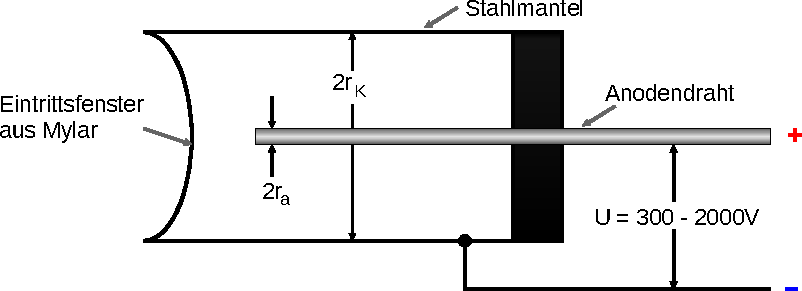
\includegraphics{figures/Abb_1.pdf}
    \caption{Querschnittdarstellung eines
    Endfenster-Zählrohrs\cite{ap03}.}
    \label{fig:abb1}
\end{figure}

Tritt nun ein geladenes Teilchen in das 
Feld ein, stößt es mit weiteren Teilchen
im Gasgemisch, bis seine Energie erschöpft ist.
Das Verhältnis der angelegten Spannung zur
Anzahl der Elektron-Ionen-Paare ist dabei in
\autoref{fig:abb2} dargestellt.

\begin{figure}[H]
    \centering
    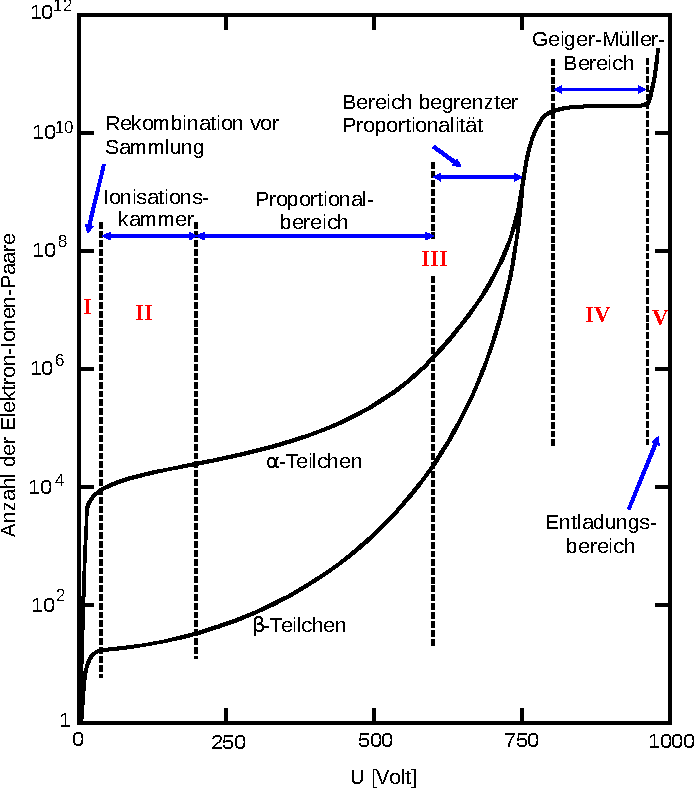
\includegraphics{figures/Abb_2.pdf}
    \caption{Anzahl der Elektron-Ionen-Paare in Abhängigkeit von der Spannung $U$\cite{ap03}.}
    \label{fig:abb2}
\end{figure}

Besitzen die einfallenden Elektronen genug
Energie, um durch Stöße im Gasgemisch weitere
Teilchen zu ionisieren, die dann, bei genügender
vorliegender Spannung, ihrerseits weitere
Teilchen ionisieren, wird von einer \textbf{Townsend-Lawine}
gesprochen. \\

Wird die Spannung noch weiter erhöht, geht,
wie in Bereich IV zu erkennnen, die
Proportionalität zwischen Elektron-Ionen-Paaren
und Spannung verloren.
Es bildet sich ein Plateau, in dem die Kurven
für $\alpha$- und $\beta$-Strahlung zusammenlaufen
und die Paaranzahl auch bei sich verändernder
Spannung konstant bleibt. \\

Aufgrund ihrer größeren Masse verbleiben die Kationen
länger im Gasraum zwischen der Anode und Kathode, sie bauen
also eine temporäre, radialsymmetrische Raumladung auf,
die das Feld in Drahtnähe soweit abschwächt,
dass neue eintreffende Teilchen nicht registriert werden.
Die Zeit vom Eintreffen eines Teilchens bis zu dem
Zeitpunkt, ab dem ein neues Teilchen erkannt werden kann,
wird als \textbf{Totzeit} bezeichnet. \\

Während die Kationenwolke abwandert, 
besitzen neue Ausgangsimpulse eine 
geringere Höhe.
Die \textbf{Erholungszeit} beschreibt also
den Zeitraum, bis die Impulshöhe wieder auf
Normalniveau ist.\\

Eine Darstellung dieser Vorgänge findet sich in
\autoref{fig:abb3}.

\begin{figure}[H]
    \centering
    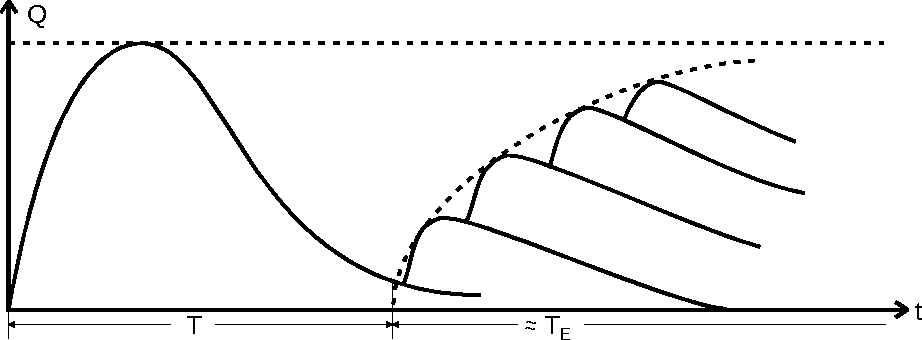
\includegraphics{figures/Abb_3.pdf}
    \caption{Tot- und Erholungszeit im Ladungs-Zeit-Diagramm\cite{ap03}.}
    \label{fig:abb3}
\end{figure}

Bei der Entladung der Ionen ist es möglich,
dass beim Auftreffen auf den Zählrohrmantel
Elektronen freigesetzt werden.
Diese Sekundärelektronen können weitere,
zeitlich versetzte Ausgangsimpulse auslösen,
die \textbf{Nachentladungen} genannt werden.
Da der zeitliche Abstand der Nachentladungen
größer als die Totzeit ist, sollten sie so weit
wie möglich reduziert werden.
Zu diesem Zweck ist das Gasgemisch oft mit
Alkoholmolekülen versetzt, die die Edelgasionen
'auffangen'. \\

Berechnen lässt sich die Totzeit dabei z.B. über die Zwei-Quellen-Methode.
Mit zwei Strahlungsquellen werden die Teilchenzahlen $N_1$, $N_2$ sowie $N_{1 + 2}$ aufgenommen.
Die Totzeit bestimmt sich dann näherungsweise über

\begin{equation}
    T \approx \frac{N_1 + N_2 - N_{1 + 2}}{2 N_1 N_2} \,.
    \label{eq:totzeit}
\end{equation} \\

Wie bereits in \autoref{fig:abb3} zu betrachten,
soll nun der als Charakteristik bezeichnete
Operationsbereich des Zählrohrs betrachtet werden. \\

Dazu sei in \autoref{fig:abb4} erneut Bereich IV dargestellt.

\begin{figure}[H]
    \centering
    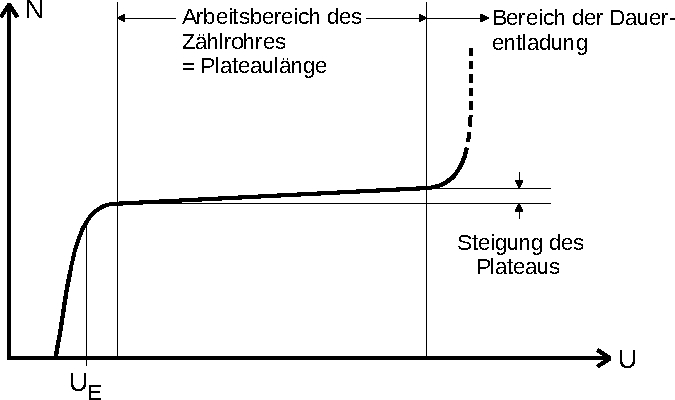
\includegraphics{figures/Abb_4.pdf}
    \caption{Zählrohrcharakteristik bei konstanter Strahlungsintensität\cite{ap03}.}
    \label{fig:abb4}
\end{figure}

Die Spannung $U_{\text{E}}$ beschreibt dabei
den Beginn des Auslösebereiches, an den das
Plateau anschließt.
Bei einem idealen Zählrohr sollte die Plateausteigung
$m = 0$ sein, in der Realität sorgen jedoch unvermeidbare
Nachentladungen dafür, dass immer eine geringe Steigung zu messen ist. \\

Am Ende des Plateaus wird die Spannung so gewaltig,
dass ein einzelnes Teilchen ausreicht, um
eine Dauerentladung auszulösen, die schnell
zur permanenten Zerstörung des Zählrohrs führen kann. \\

Die pro Teilchen freigesetzte Ladung $\Delta Q$ in einem Zeitintervall $\Delta t$ bei einer Teilchenzahl $N$ kann dabei aus
\begin{equation}
    I = \frac{\Delta Q}{\Delta t} N
    \label{eq:teilchenstrom}
\end{equation}
bestimmt werden.


% Ende Theorie
